
\begin{frame}{Child-Langmuir Law}

\begin{columns}
  \begin{column}{0.45\linewidth}
    For two plates:
    \begin{itemize}
      \item area $A$
      \item separated by $d$
      \item potential difference $V_a$
    \end{itemize} the limiting current is given by:
  \end{column}
  \begin{column}{0.45\linewidth}
    \begin{figure}
      \centering
      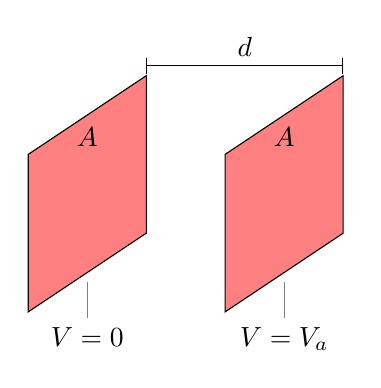
\begin{tikzpicture}
        \draw [fill=red!50]
          (0,0)
          -- node[below=1]{$A$}
            node(plate1)[above,pos=1]{}
            ++(1.5,1)
          -- ++(0,-2)
          -- node[pin={below:$V=0$}]{} ++(-1.5,-1)
          -- cycle
        ;
        \draw [fill=red!50]
          (2.5,0)
          -- node[below=1]{$A$}
            node(plate2)[above,pos=1]{}
            ++(1.5,1)
          -- ++(0,-2)
          -- node[pin={below:$V=V_a$}]{} ++(-1.5,-1)
          -- cycle
        ;
        \draw[|-|]
          (plate1.center)
          -- node[above]{$d$} (plate2.center);
      \end{tikzpicture}
    \end{figure}
  \end{column}
\end{columns}
\begin{block}{Child-Langmuir Law}
  \begin{equation*}
    I_a  = JA = \frac{4 \varepsilon_0}{9}\sqrt{\frac{2 e}{m_e} } \frac{A V_a^{3/2}}{d^2}
  \end{equation*}
\end{block}
\end{frame}

\begin{frame}{Quantum Step Approximation}
	\begin{columns}
	\begin{column}{.48 \linewidth}
    We have the relations:
    	\begin{itemize}
          \item $ k_{0 \smallT} = k_{1 \smallT} $
          \item<2-> Trigonometric Identities
          \item<3-> 1D Transmission result: \\ $ T(k(E),\theta) =
          \frac{4 k_{0 z} k_{1 z}}{ \left ( k_{0 z} + k_{1 z} \right ) ^{2} } $
        \end{itemize}    
  	\end{column}
	\begin{column}{.52 \linewidth}
    	\begin{figure}[H]
          	\centering
        	\shadowbox
        	{
        	\only<article| beamer>{
        	\only<1-3>{
        	\includegraphics{quantum_step}
        	}}
        	\only<presentation>{
        	\only<4->{
        	\includegraphics[scale=0.7]{quantum_step}}
        	}}
        	\only<article>{\caption{Quantum Step Potential}}
        \end{figure}
    \end{column}
	\end{columns}
\only<4->
{
    \begin{block}{Resulting Transmission Function}
        \begin{equation*}
           	T(E,\theta) = \frac{4 \sqrt{E} \cos \theta \sqrt{E \cos^{2} \theta
           	+ V } }{ \left ( \sqrt{E} \cos \theta + \sqrt{E \cos^{2} \theta
           	+ V } \right )^{2} }
    	\end{equation*}
		\center{In terms of exit energy $E$ and exit angle $\theta$}
    \end{block}
}
\end{frame}

\begin{frame}{Photoemission from Flat Metal}
  \begin{columns}
  \begin{column}{0.54\linewidth}
  \begin{center}
  \begin{tikzpicture}
    \filldraw
      [fill=black!50]
      (0,0) 
      node [name=photocathode1,below right]{}
      node [below=1mm of photocathode1] {}
      -- ++(1,0)
      -- ++(0,-5)
      node [name=source,midway] {} 
      -- ++(-1,0)
      -- cycle
    ;
    \draw
      [-latex,ultra thick,green] 
      ($(source) + (45:3.5)$) 
      -- (source.east)
      node [name=laser label,pos=0.3,black,fill=white] {Laser ($\lambda$)}
    ;
    \fill
      [blue!30]
      (source.east)
      -- ++(3,6mm)
      -- ++(0,-12mm)
      -- cycle
    ;
    \draw
      [-latex,ultra thick,blue]
      (source.east)
      -- ++(3,6mm)
    ;
    \draw
      [-latex,ultra thick,blue]
      (source.east)
      -- ++(3,-6mm)
      node [name=electron label,at end,black,below,align=center]{Photoemitted\\Electrons}
    ;
    \draw
      [dashed]
      (source)
      -- ++(4,0)
    ;
%     \draw 
%       ($(source) + (1,0)$) 
%       arc (0:41:1)
%       node [right=0.3] {$\theta$}
%     ;
  \end{tikzpicture}
  \end{center}
  \end{column}
  \begin{column}{0.44\linewidth}
    \begin{equation*}
      P(\theta) = \smashoperator{\int\limits_{0}^{\Delta E = \hbar \omega - \Phi}} T(E,\theta) \dx{E}
    \end{equation*}
    \centerline{\tiny Assuming flat Fermi function}
    \begin{figure}
      \centering
      \includegraphics[width=0.9\linewidth]{Angle}
    \end{figure}
  \end{column}
  \end{columns}
\end{frame}

\begin{frame}{Emission Probability vs. Excess Energy}
  \begin{columns}
    \begin{column}{0.49\linewidth}
      %Angularly-integrated Emission Probability
      \begin{equation*}
        P(E) = \int\limits_0^E \int\limits_{-\pi/2}^{-\pi/2} T(E_0,\theta) \dx{\theta}\dx{E_0}
      \end{equation*}
    \end{column}
    \begin{column}{0.49\linewidth}
      \begin{figure}
        \centering
        \includegraphics[width=0.9\linewidth]{Energy}
      \end{figure}
    \end{column}
  \end{columns}
  
\end{frame}

\begin{frame}{Gaussian Distribution}
If we define our distribution of electrons in the pulse as:
	\begin{multline*}
		f \left ( x , y , z , p_{x} , p_{y} , p_{z} \right ) = \\ \frac{N}{ \left ( 2 \pi \right )^{3} \sigma_{ \smallT } \eta_{ \scriptscriptstyle T } \sqrt{ \sigma_{z} \eta_{z}} } \exp \Biggl [ - \biggl ( \frac{x^{2}} {2 \sigma_{ \smallT }} + \frac{y^{2}} {2 \sigma_{ \smallT }} + \frac{z^{2}} {2\sigma_{z}} + \\ \frac{ \left ( p_{x} - \dfrac{\gamma_{ \smallT } x} {\sigma_{ \smallT }} \right )^{2}} {2 \eta_{ \smallT }} + \frac{ \left ( p_{y} - \dfrac{\gamma_{ \smallT } y} {\sigma_{ \smallT }} \right )^{2}} {2 \eta_{ \smallT }} + \frac{ \left (p_{z} - \dfrac{\gamma_{z} z} {\sigma_{z}} \right )^{2}} {2 \eta_{z}} \biggr ) \Biggr ]
	\end{multline*}
N.B. the coefficient allows $ \int f d\vec{r} d\vec{p} = N $

\end{frame}

\begin{frame}{What Are These Parameters?}
	\begin{columns}
		\begin{column}{2in}
			\begin{itemize}[<+->]
				\item $ \sigma_{i} \Rightarrow$ spatial variance
				\item $ \eta_{i} \Rightarrow$ \emph{local} momentum variance
				\item $ \gamma_{i} \Rightarrow$ spatial variation of the local momentum variance (chirp)
			\end{itemize}
		\end{column}
		\begin{column}{2in}
			\begin{figure}
				\includegraphics<1>{Gaussian1.jpg}
				\includegraphics<2>{Gaussian2.jpg}
				\includegraphics<3>{Gaussian3.jpg}
			\end{figure}
		\end{column}
	\end{columns}
\end{frame}

\begin{frame}{AG Model Equations}
\begin{block}{Michalik and Sipe equation set}
	\begin{gather*}
		\frac{d\sigma_{i}} {dt} = \frac{2} {m} \gamma_{i} \\
		\frac{d \gamma_{i}} {dt} = \frac{1} {m} \left (\eta_{i} + \frac{\gamma_{i}^{2}} {\sigma_{i}} \right ) + \frac{1} {4 \pi \epsilon_{0}} \frac{N e^{2}} {6 \sqrt{\sigma_{i} \pi} } L_{i}(\xi) \\
		\frac{d\eta_{i}} {dt} = - \frac{2 \gamma_{i} \eta_{i}} {m \sigma_{i}}
	\end{gather*}
\end{block}
\begin{itemize}
  \item $L_i(\xi)$ are well-behaved smooth functions of $\xi=\sqrt{ \sigma_{z} / \sigma_{t} }$
  \item Solve to classical Gaussian when $ N = 0 $
\end{itemize}
\end{frame}

\begin{frame}{Building the Model}

\begin{columns}
	\begin{column}{.52 \linewidth}
	\begin{itemize}
  		\item<1-> Start with the fastest electron
  		\item<2-> $ v_{fastest} = \sqrt{2 q \Delta E / m } $ \\ $ \Delta E $ is
  		excess photoemission energy
  		\item<3-> Propagate with \\ $ z_{max} = v_{fastest} t_{total} + q E t_{
  		total }^{2} / 2 m $
  		\item<4-> This is the maximum possible range
  		\item<5-> Subdivide the preceding space for future reference
	\end{itemize}
	\end{column}
	
	\begin{column}{.44 \linewidth}
    \begin{overlayarea}{.44 \linewidth}{2.1in}
    \begin{figure}[H]
    	\centering
    	\only<beamer>
    	{
    	\only<1-2>{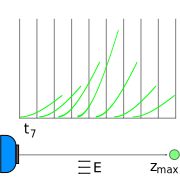
\includegraphics{bin}}
    	\only<3-4>{\includegraphics{bin1}}
    	}
    	\only<presentation>{\only<5->{\includegraphics{bin2}}}
    \end{figure}
    \end{overlayarea}
    \end{column}
\end{columns}

\end{frame}

\begin{frame}{Running the Model}

\begin{columns}
	\begin{column}{.52 \linewidth}
	\begin{itemize}
      \item<1-> At each timestep $t_{i}$ label bins by equivalent velocities
      \item<2-> $ v_{ bin } = \frac{ z_{ bin } }{ t_{ i } } - \frac{q E t_{i} }{
      2 m } $ \\ where $ t_{i} =  t_{ total } - i \delta t $
      \item<3-> This allows the velocity distribution to be superimposed
      \item<10-> After all the timesteps the number and velocity distribution
      in each bin can be computed
    \end{itemize}
	\end{column}

	\begin{column}{.44 \linewidth}
    \begin{overlayarea}{.44 \linewidth}{2.1in}
	\begin{figure}[H]
    	\centering
    	\only<beamer>
    	{
    	\only<1-2>{\includegraphics{bin2}}
    	\only<3>{\includegraphics{bin3}}
   	    \only<4>{\includegraphics{bin4}}
    	\only<5>{\includegraphics{bin5}}
    	\only<6>{\includegraphics{bin6}}
    	\only<7>{\includegraphics{bin7}}
    	\only<8>{\includegraphics{bin8}}
    	}
    	\only<9->{\includegraphics{bin9}}
    	\only<article>
    	{
    	\caption{Overlay of time slices of distributions of electrons in space bins}
    	}
    \end{figure}
	\end{overlayarea}
	\end{column}
\end{columns}

\end{frame}

\begin{frame}{Comparison with Sipe Model}
\begin{columns}
	\begin{column}{3in}
	\begin{figure}[H]
    	\centering
		\includegraphics{Acc}
		\only<article>{\caption{Acceleration dominated case}}
	\end{figure}
	\end{column}

	\begin{column}{.38 \linewidth}
		\begin{block}{For operating conditions:}    
			$ qE/m >> v_{max}/t_{total} $
		\end{block}

		\vf
 
		\only<2->
		{
		For a majority of electrons the allowed fit is reasonable
		}

    \end{column}
\end{columns}
\end{frame}

\begin{frame}
\only<presentation>{\frametitle{Comparison with Sipe Model}}
\begin{columns}

	\begin{column}{.38 \linewidth}
		\begin{block}{For operating conditions:}    
			$ qE/m << v_{max}/t_{total} $
		\end{block}

		\vf
 
		\only<2->
		{
		In this case, the fit for ``local momentum width'' (related to
		$\eta$) not very good
		}

    \end{column}

	\begin{column}{3in}
	\begin{figure}[H]
    	\centering
		\includegraphics{Vmax}
		\only<article>{\caption{Vmax dominated case}}
	\end{figure}
	\end{column}

\end{columns}
\end{frame}

\begin{frame}
\only<presentation>{\frametitle{Comparison with Sipe Model}}
\begin{columns}
	\begin{column}{3in}
	\begin{figure}[H]
  		\centering
		\includegraphics{Equal}
		\only<article>{\caption{Case where Vmax and Acceleration are approximately equal}}
	\end{figure}
	\end{column}

	\begin{column}{.38\linewidth}
		\begin{block}{For operating conditions:}    
			$ qE/m \approx v_{max}/t_{total} $
		\end{block}

		\vf
 
		\only<2->
		{
		Even this more intermediate case will still have some artifacts
		owing to the limitations of the model
		}

    \end{column}
\end{columns}
\end{frame}

\begin{frame}{Regenerative Laser Amplifier}
  Regenerative laser amplifier:
  \begin{columns}
    \begin{column}{0.49\linewidth}
      \begin{itemize}
        \item 650Hz
        \item 100$\mu$J fundamental
        \item<2-> [$\hookrightarrow$] Generates $10^8$ electrons
        \begin{itemize}
          \item<3-> Single-shot imaging
          \item<4-> Observe charge-charge interaction
          \item<5-> Investigate short-pulse Child's Law
        \end{itemize}
      \end{itemize}
    \end{column}
    \begin{column}{0.49\linewidth}
    \begin{center}
      \includegraphics{regen}
    \end{center}
    \end{column}
  \end{columns}
\end{frame}

\begin{frame}{Two-photon Assisted Thermionic Emission (2PTE)}
  \begin{center}
    \input{au_plot}
  \end{center}
\end{frame} 
